\section{熱真空試験(中村・坂本)}

ウェルリサーチ社(千葉県)において,以下を実施した.それぞれの試験の詳細については実験計画書を参照.

\begin{itemize}
	\item 2018年2月13~14日(2日間) EM熱平衡試験:熱解析モデルのコリレーション「OP-S1-0080 EM熱平衡試験計画書・手順書」
	\item 2018年2月27~3月1日(3日間) EM 3U熱真空試験:膜展開前のコンフィグでの機器動作確認「OP-S1-0081 EM熱真空試験計画書・手順書」
	\item 2018年3月12~14日(3日間) EM 2U熱真空試験:膜展開部がバス部から離れたコンフィグでの機器動作確認「OP-S1-0083 EM2U熱真空試験計画書・手順書」
	\item 2018年9月25~27日(3日間) FM熱真空試験:FM膜展開前のコンフィグでの機器動作確認「OP-S1-0061 FM熱真空試験計画書・手順書」
\end{itemize}

EMを用いた熱真空試験の前には適切にベーキングを実施しなかったため,熱真空槽を汚してしまった可能性がある.FMでの熱真空試験の前には,
まずFM展開膜のみ摂氏60度で24時間,サカセアドテックの真空オーブン内でベーキングを行った(真空度29.3~29.6in.Hg).これはダミーデバイスの接着に用いたエルファンのアウトガスが特に多いことを懸念したためである
(他の材料より1桁多い).
その後,FM組み立てを実施してからウェルリサーチ社の恒温槽を用いて摂氏60度24時間のベーキングを実施した.

\subsection{EM熱平衡試験(2018年2月13~14日)}

供試体の概要と,試験の写真を示す.
\begin{figure}[H]
		\centering
		    \begin{tabular}{cc}
	 \begin{minipage}{0.5\hsize}
		\begin{center}
			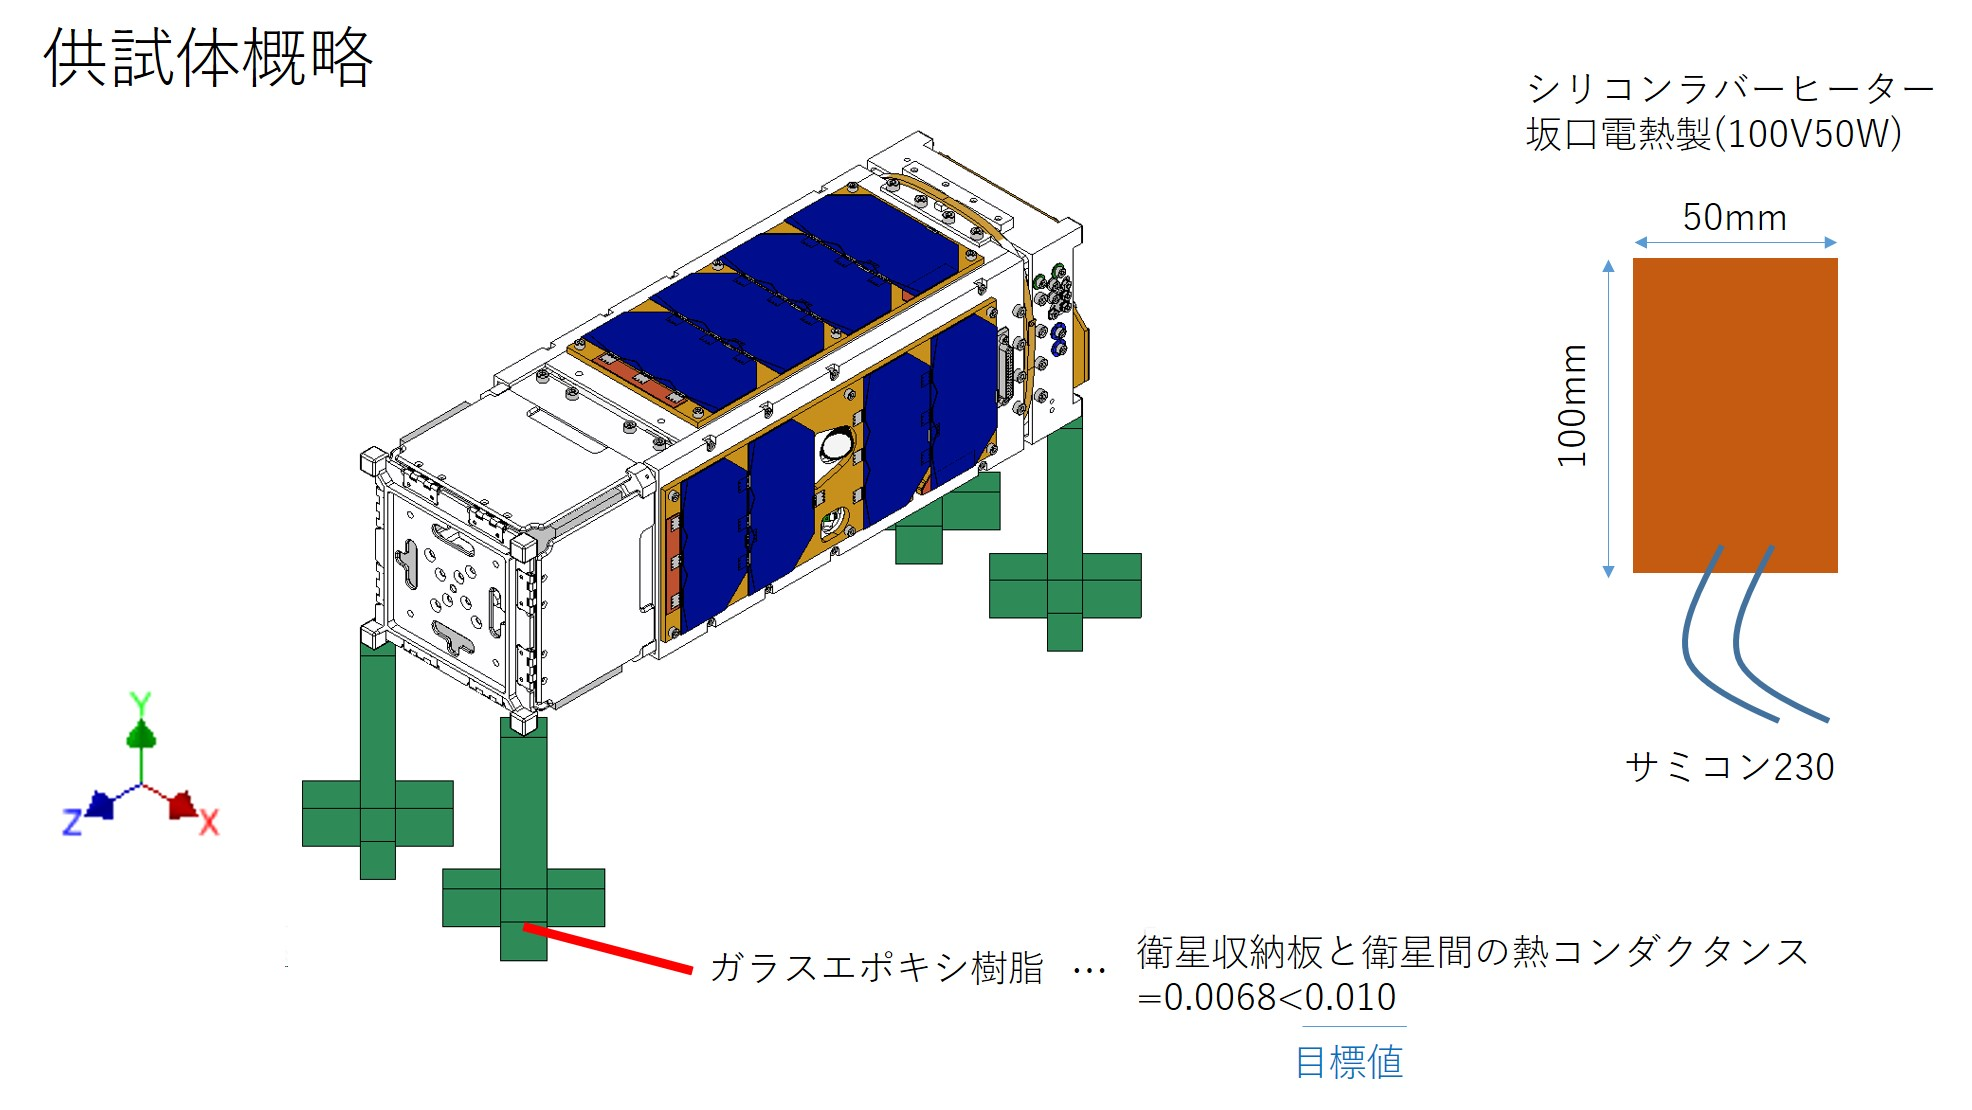
\includegraphics[width=1\textwidth]{04/fig/4-8-1-1.jpg}
		\end{center}
	\end{minipage}&
	\begin{minipage}{0.5\hsize}
		\begin{center}
			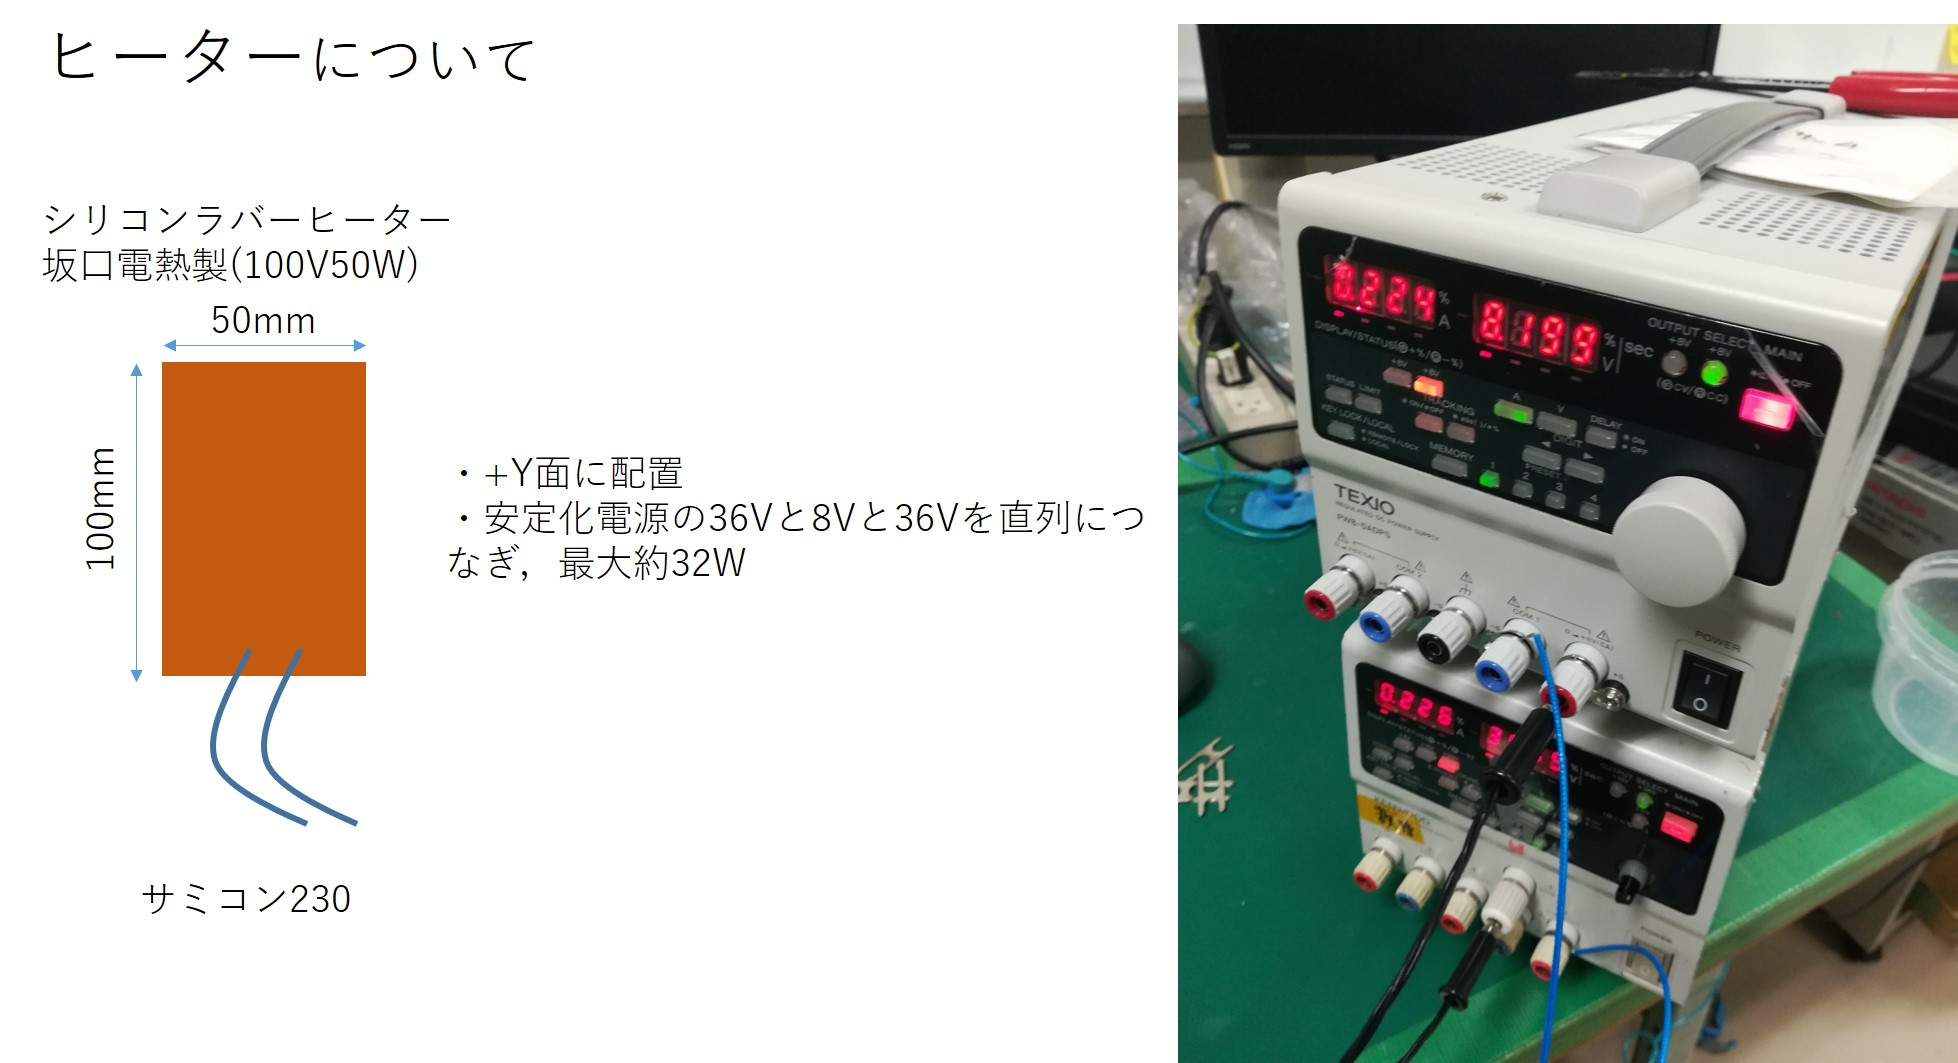
\includegraphics[width=1\textwidth]{04/fig/4-8-1-2.jpg}
		\end{center}
	\end{minipage}\\
	 \begin{minipage}{0.5\hsize}
	\begin{center}
		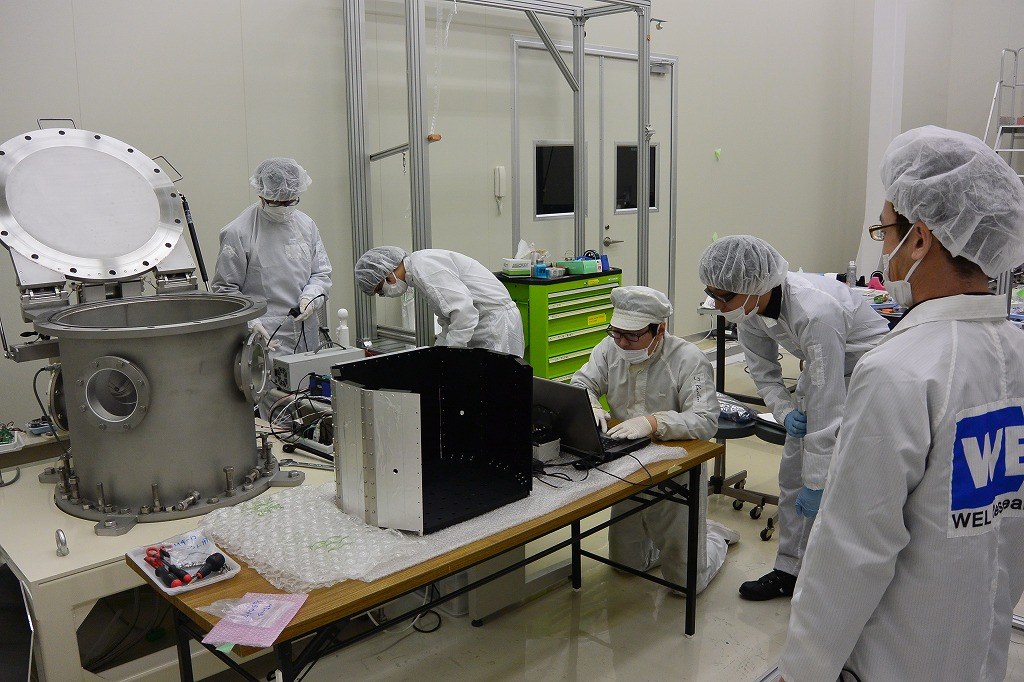
\includegraphics[width=1\textwidth]{04/fig/4-8-1-3.jpg}
	\end{center}
\end{minipage}&
\begin{minipage}{0.5\hsize}
	\begin{center}
		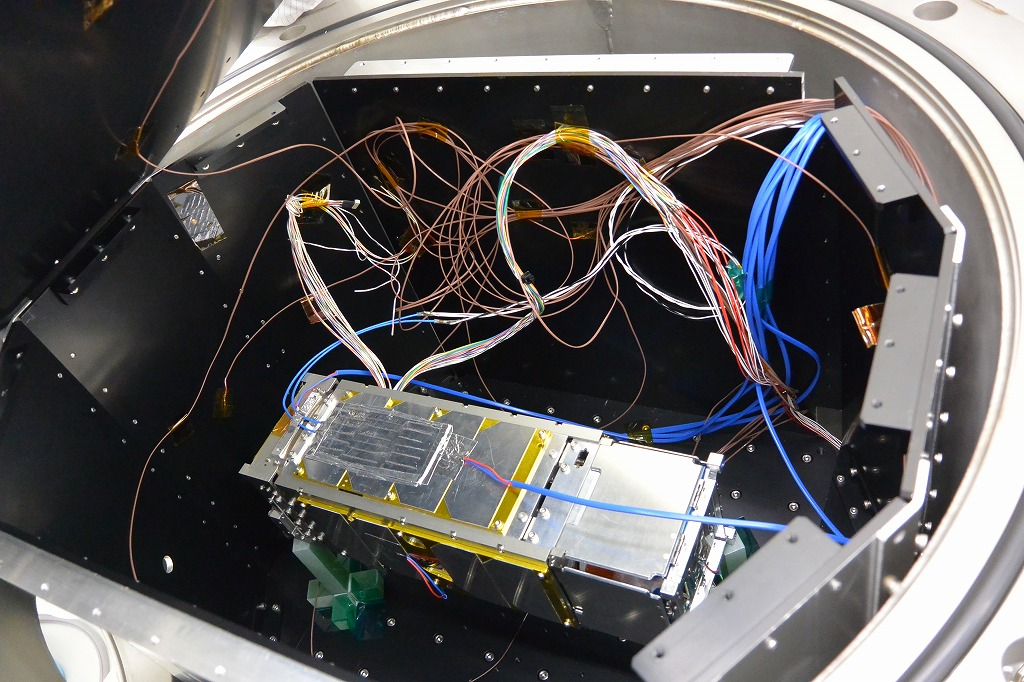
\includegraphics[width=1\textwidth]{04/fig/4-8-1-4.jpg}
	\end{center}
\end{minipage}
\end{tabular}
		\caption{EM熱平衡試験(2018年2月13~14日)}
	\label{fig4-8-1-1}
\end{figure}

\subsection{EM 3U熱真空試験(2018年2月27~3月1日)}

摂氏30度,-25度,-35度での試験を実施した.以下に機能確認項目を示す.

\begin{figure}[H]
	\centering
				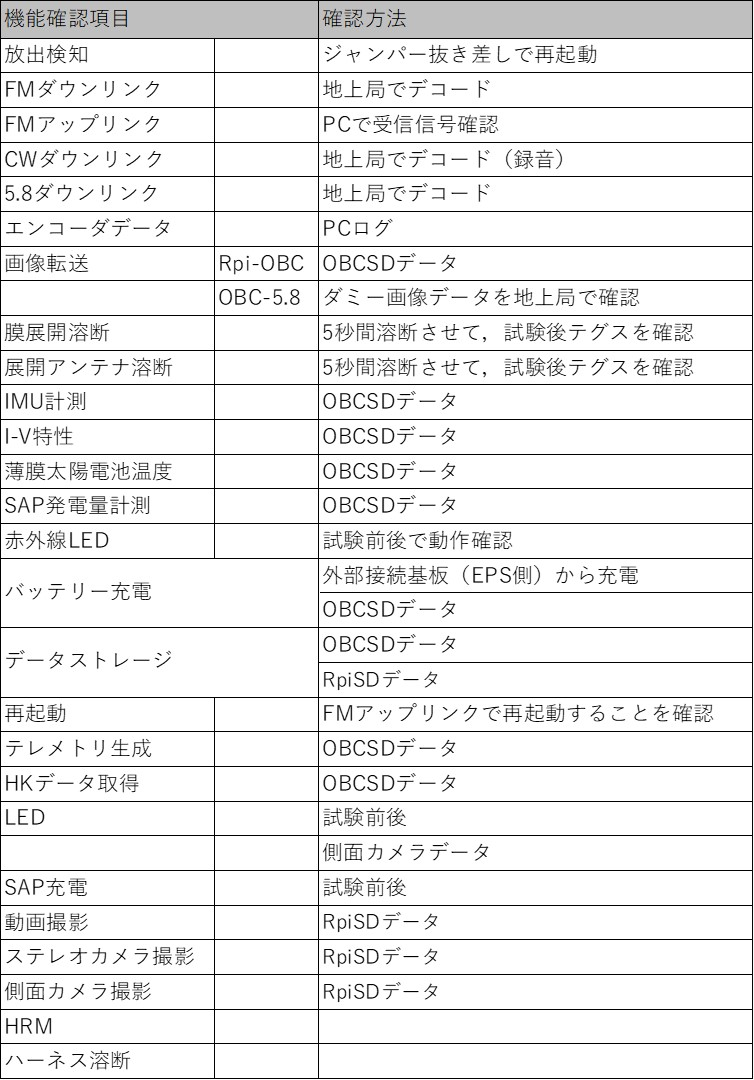
\includegraphics[width=.5\textwidth]{04/fig/4-8-2-1.jpg}
		\caption{EM 3U熱真空試験(2018年2月27~3月1日)機能確認項目}
	\label{fig4-8-2-1}
\end{figure}

\subsection{EM 2U熱真空試験(2018年3月12~14日)}

膜展開部がバス部から離れたコンフィグレーションを模擬した.
摂氏30度,-25度,-35度での試験を実施した.写真を以下に示す.
\begin{figure}[H]
	\centering
	\begin{tabular}{cc}
		\begin{minipage}{0.5\hsize}
			\begin{center}
				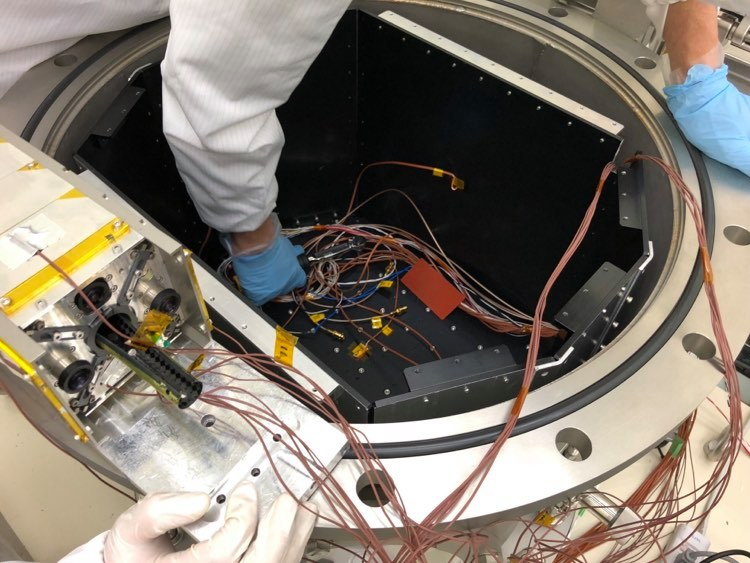
\includegraphics[width=1\textwidth]{04/fig/4-8-3-1.jpg}
			\end{center}
		\end{minipage}&
		\begin{minipage}{0.5\hsize}
			\begin{center}
				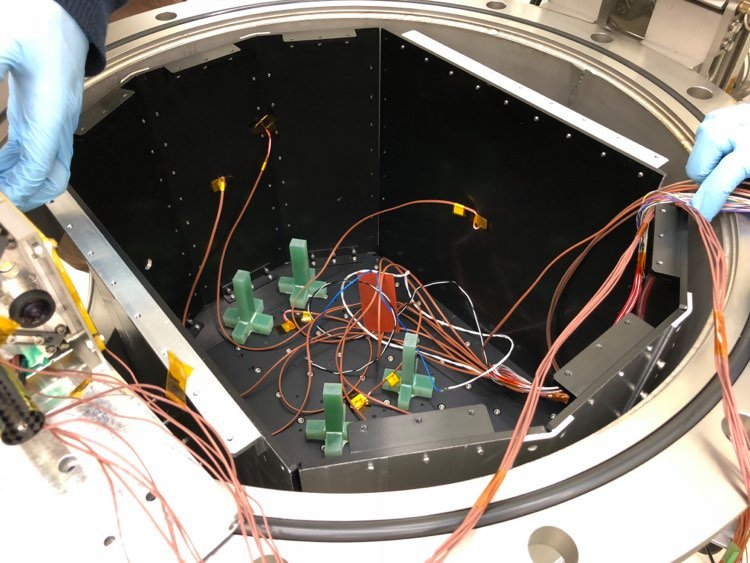
\includegraphics[width=1\textwidth]{04/fig/4-8-3-2.jpg}
			\end{center}
		\end{minipage}\\
		\begin{minipage}{0.5\hsize}
			\begin{center}
				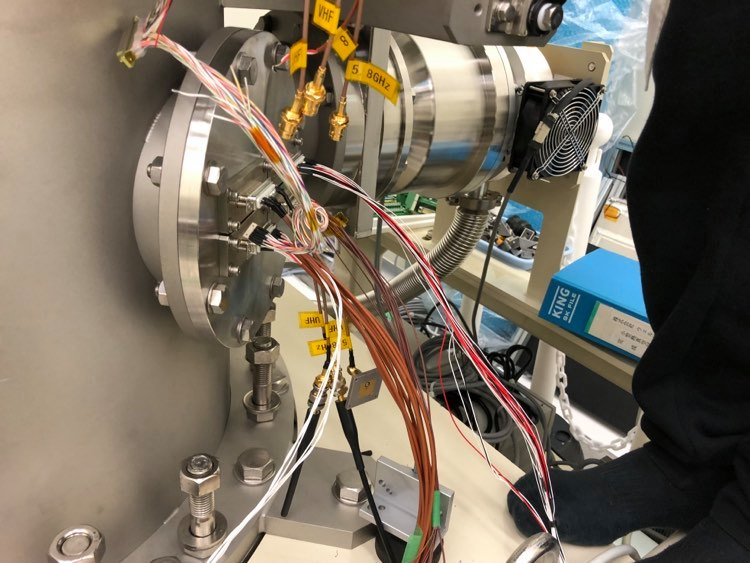
\includegraphics[width=1\textwidth]{04/fig/4-8-3-3.jpg}
			\end{center}
		\end{minipage}&
		\begin{minipage}{0.5\hsize}
			\begin{center}
				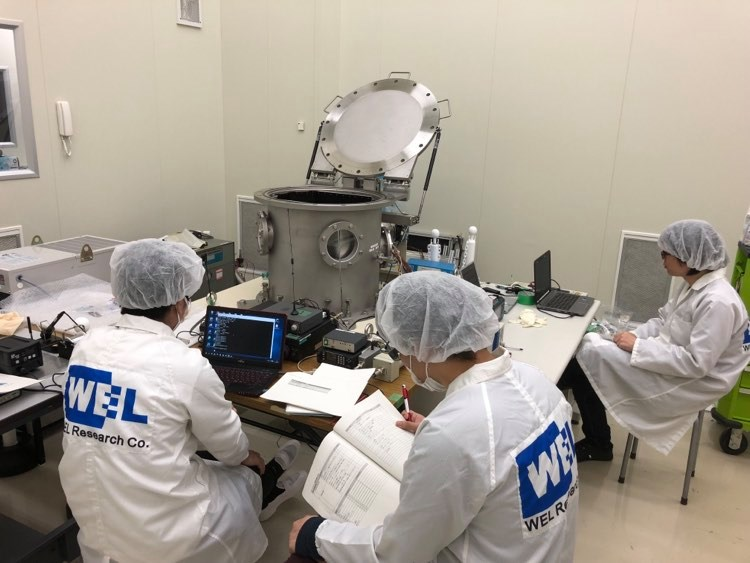
\includegraphics[width=1\textwidth]{04/fig/4-8-3-4.jpg}
			\end{center}
		\end{minipage}
	\end{tabular}
	\caption{EM 2U熱真空試験(2018年3月12~14日)}
	\label{fig4-8-3-1}
\end{figure}

\subsection{FM熱真空試験(2018年9月25~27日)}

FMについて,膜展開前のコンフィグでの動作確認を実施した.
摂氏30度,-25度,-35度での試験を実施した.写真を以下に示す.
\begin{figure}[H]
	\centering
	\begin{tabular}{cc}
		\begin{minipage}{0.5\hsize}
			\begin{center}
				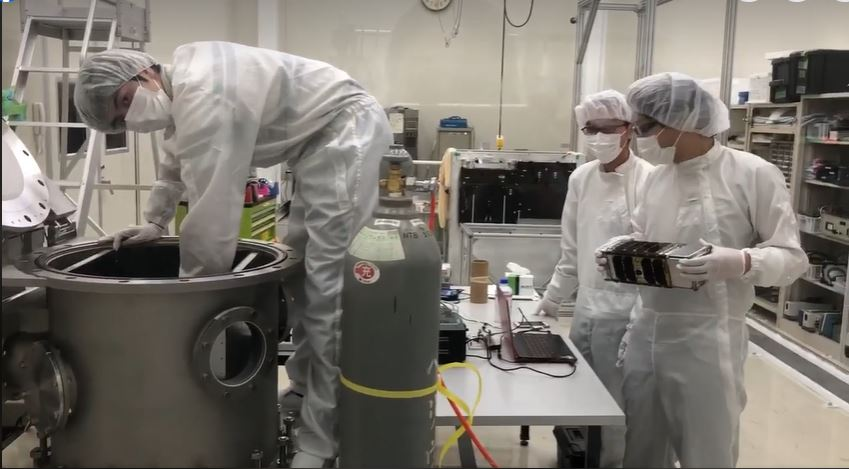
\includegraphics[width=1\textwidth]{04/fig/4-8-4-1.jpg}
			\end{center}
		\end{minipage}&
		\begin{minipage}{0.5\hsize}
			\begin{center}
				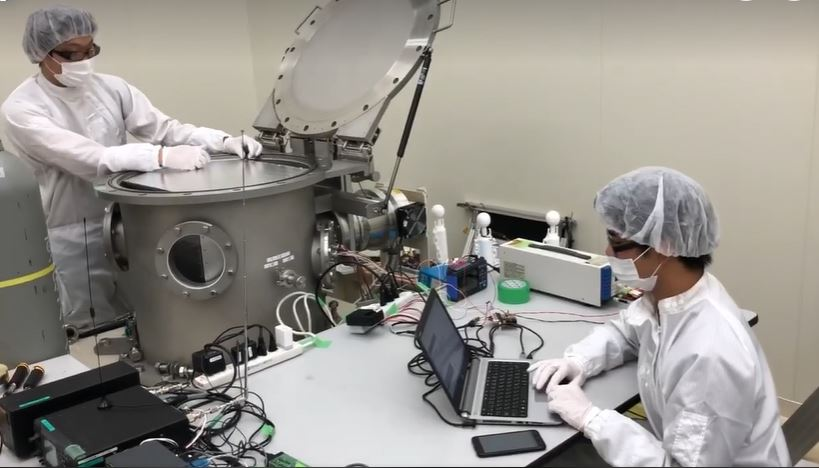
\includegraphics[width=1\textwidth]{04/fig/4-8-4-2.jpg}
			\end{center}
		\end{minipage}\\
		\begin{minipage}{0.5\hsize}
			\begin{center}
				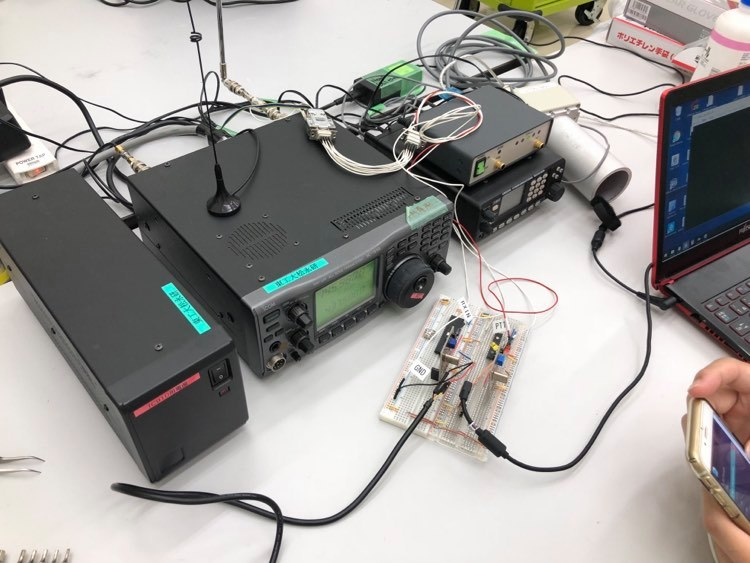
\includegraphics[width=1\textwidth]{04/fig/4-8-4-3.jpg}
			\end{center}
		\end{minipage}&
		\begin{minipage}{0.5\hsize}
			\begin{center}
				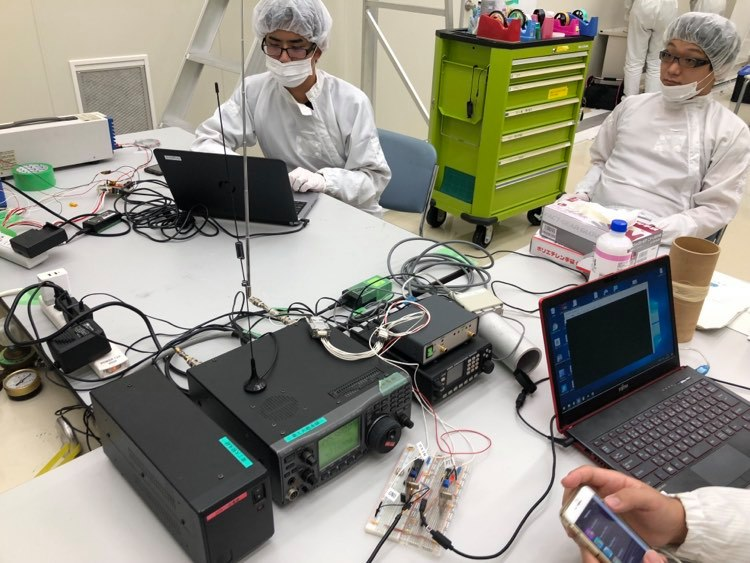
\includegraphics[width=1\textwidth]{04/fig/4-8-4-4.jpg}
			\end{center}
		\end{minipage}
	\end{tabular}
	\caption{FM熱真空試験(2018年9月25~27日)}
	\label{fig4-8-4-1}
\end{figure}

\subsection{熱真空試験での気づき}
FM熱真空試験中(およびFM振動試験前後)の機能試験において,5.8GHzの通信成立を音だけで確認して文字列をターミナルで確認することを怠っていたため,これらの試験後に5.8GHzの通信不具合に気付くことになり,いちど機体を分解する大きな手戻りが発生した.手戻りが生じない機能試験方法を取るべきだった.

また,小型の衛星に対して熱電対の配線が全体を取り囲むようなセッティングとなり,配線を通した熱伝導の影響がどの程度あったかが不明で,熱平衡試験の精度について不明点が多い.結果として熱解析結果より軌道での衛星温度は高めであったので,熱解析および熱平衡試験がじゅうぶんに適切ではなかった可能性がある.

長時間にわたって熱真空槽を貸して下さったウェルリサーチ社の皆様に感謝するとともに,幾夜を超える試験を実施した開発メンバーの労を労いたい.